\documentclass{article}


% if you need to pass options to natbib, use, e.g.:
%     \PassOptionsToPackage{numbers, compress}{natbib}
% before loading neurips_2023


% ready for submission
\usepackage[preprint]{neurips_2023}
\usepackage{notation}


% to compile a preprint version, e.g., for submission to arXiv, add add the
% [preprint] option:
%     \usepackage[preprint]{neurips_2023}


% to compile a camera-ready version, add the [final] option, e.g.:
%     \usepackage[final]{neurips_2023}


% to avoid loading the natbib package, add option nonatbib:
%    \usepackage[nonatbib]{neurips_2023}


\usepackage[utf8]{inputenc} % allow utf-8 input
\usepackage[T1]{fontenc}    % use 8-bit T1 fonts
\usepackage{hyperref}       % hyperlinks
\usepackage{url}            % simple URL typesetting
\usepackage{booktabs}       % professional-quality tables
\usepackage{amsfonts}       % blackboard math symbols
\usepackage{nicefrac}       % compact symbols for 1/2, etc.
\usepackage{microtype}      % microtypography
\usepackage{xcolor}         % colors

\usepackage{graphicx}
\usepackage{mathtools}

\usepackage{algorithm}
\usepackage{algorithmicx}
\usepackage{algpseudocode}

\renewcommand{\algorithmicrequire}{\textbf{Input:}}
\renewcommand{\algorithmicensure}{\textbf{Output:}}

\newtheorem{definition}{Definition}

\title{Generative models based on ODE and SDE}


% The \author macro works with any number of authors. There are two commands
% used to separate the names and addresses of multiple authors: \And and \AND.
%
% Using \And between authors leaves it to LaTeX to determine where to break the
% lines. Using \AND forces a line break at that point. So, if LaTeX puts 3 of 4
% authors names on the first line, and the last on the second line, try using
% \AND instead of \And before the third author name.


\author{%
  Denis Rakitin\\
  \texttt{rakitindenis32@gmail.com} \\
  % examples of more authors
  % \And
  % Coauthor \\
  % Affiliation \\
  % Address \\
  % \texttt{email} \\
  % \AND
  % Coauthor \\
  % Affiliation \\
  % Address \\
  % \texttt{email} \\
  % \And
  % Coauthor \\
  % Affiliation \\
  % Address \\
  % \texttt{email} \\
  % \And
  % Coauthor \\
  % Affiliation \\
  % Address \\
  % \texttt{email} \\
}


\begin{document}


\maketitle


% \begin{abstract}
%   The abstract paragraph should be indented \nicefrac{1}{2}~inch (3~picas) on
%   both the left- and right-hand margins. Use 10~point type, with a vertical
%   spacing (leading) of 11~points.  The word \textbf{Abstract} must be centered,
%   bold, and in point size 12. Two line spaces precede the abstract. The abstract
%   must be limited to one paragraph.
% \end{abstract}

\tableofcontents

\newpage

\section{Introduction}
\begin{figure}[h]
\centering
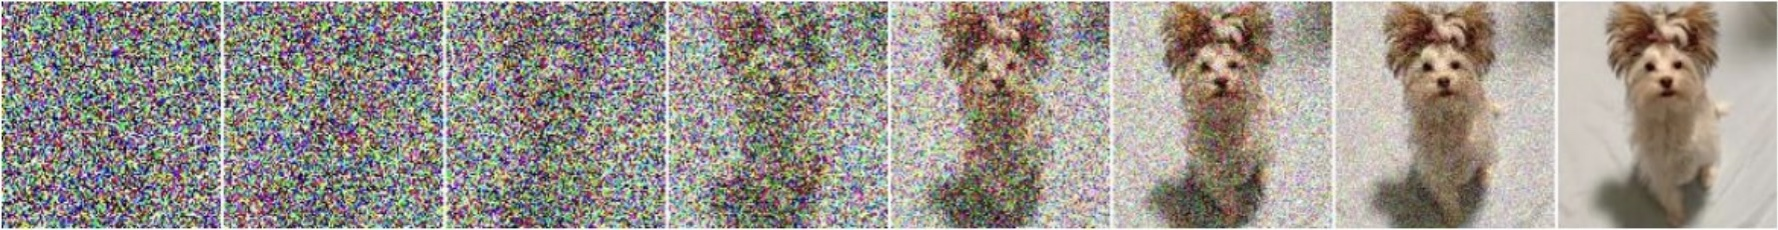
\includegraphics[width=\textwidth]{images/diffusion.png}
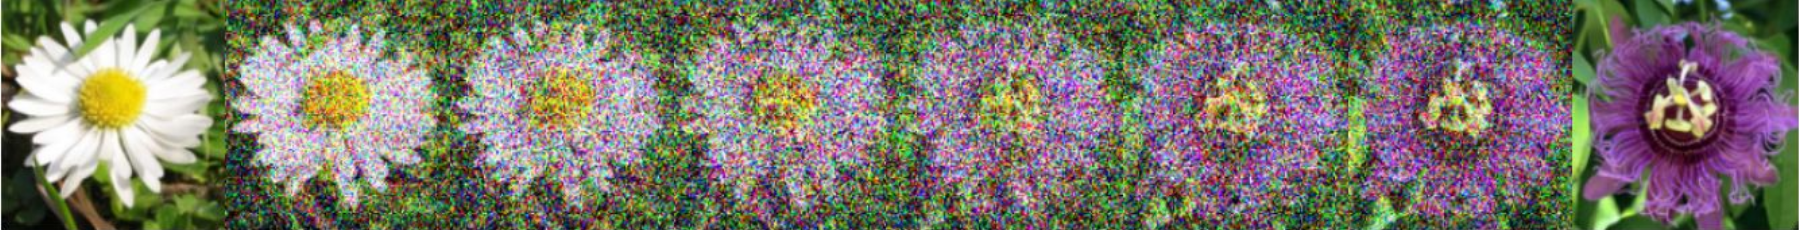
\includegraphics[width=\textwidth]{images/bridge.png}
\caption{Top: denoising process, defined by a diffusion model~\cite{song2020score}. Bottom: stochastic interpolation between two pictures~\cite{albergo2023stochastic}.}
\end{figure}

This tutorial aims to introduce the reader to the mathematical methods which are widely used in contemporary generative modeling. Big practical success of diffusion models~\cite{ho2020denoising, de2021diffusion, song2020score}, which generate a sequence of pictures instead of just the target one, led to development of a novel family of models that describe some dynamic processes. Almost all processes occuring in the real world can be described by differential equations, which will be the basis of the generative models reviewed here. We will cover methods based on either ordinary (ODE) or stochastic (SDE) differential equations, applicable for generation~\cite{song2020score, lipman2022flow, tong2023conditional, albergo2022building, albergo2023stochastic}, paired~\cite{tong2023conditional, albergo2022building, albergo2023stochastic, liu20232} and unpaired~\cite{liu2022flow, shi2023diffusion, korotin2022neural, gushchin2022entropic} domain translation, formalized as an instance of the optimal transport problem.

\section{Diffusion models} Generally speaking, diffusion models define a process of step-by-step noising of a picture and try to learn the reverse process, which allows to generate new images starting with a pure noise. There are different approaches for formalizing this concept. The earlier score-based models as NCSN~\cite{song2019generative} learn score functions of probability distributions at all noise levels and sample with a consequent Langevin dynamics~\cite{welling2011bayesian} going from larger to smaller noise levels. In \cite{ho2020denoising} the backward denoising process is trained as a latent variable model with a variational distribution on noisy images, corresponding to a forward noising process. Finally, the authors of~\cite{song2020score} consider a continuous-time noising SDE and construct the reverse, which can be seen as a unifying framework for previous approaches. On the one hand, the backward SDE explicitly requires knowing score functions at all noise levels, which is similar to the earlier score-based models. On the other hand, discrete-time sampling schemes from the backward SDE result in a discrete-time process very similar to the one in~\cite{ho2020denoising}. In this section, we will cover the original score-based approach and models, based on SDE.

\subsection{Score-based models}
The general problem of generative modeling consists of constructing the probabilistic model $p_\theta$ given a data set $X_1, \ldots, X_n \sim p_{data}$ in such a way that $p_\theta \approx p_{data}$. 

There are mainly 3 families of non-diffusion generative models: Generative Adversarial Networks  (GANs)~\cite{goodfellow2014generative}, Variational Autoencoders (VAEs)~\cite{kingma2013auto} and Normalizing Flows (NFs)~\cite{dinh2014nice,rezende2015variational}. Despite different training procedures, all of them share the same simple generation scheme: picture $x$ is obtained by transforming noise $z$ by a trained network $G_\theta$: $x = G_\theta(z)$. In contrast, score-based models do not learn the generator explicitly, but try to approximate the score function of the distribution: $s_\theta(x) \approx \nabla_{x} \log p_{data}(x)$. But why is this statistic valuable?

First, it can be used for finding mode of the distribution by gradient ascent: if 
\[
    X_{t + 1} = X_t + \gamma \nabla \log p_{data}(X_t),
\]
then
\[
    X_t \xrightarrow[t \rightarrow \infty]{} x* = \arg\max\limits_{x} \log p_{data}(x) = \arg\max\limits_{x} p_{data}(x).
\]
Of course, in general multi-modal case method converges to one of the stationary points of $\log p_{data}(x)$.

Furthermore, it can be used to obtain samples from the distribution using Langevin dynamics~\cite{welling2011bayesian}:
\[
    X_{t + 1} = X_t + \gamma \nabla \log p_{data}(X_t) + \sqrt{2 \gamma} \, \varepsilon_t,
\]
where $\varepsilon_t \sim \mathcal{N}(0, I)$ is independent with $X_t$. In regular cases, one can prove that 
\[
    p_{X_t} \xrightarrow[t \rightarrow \infty]{} p^{\gamma},
\]
where $p^{\gamma}$ is a distribution close to $p_{data}$ that depends on a discretizarion step and converges to $p_{data}$, when $\gamma$ converges to zero:
\[
    p^{\gamma} \xrightarrow[\gamma \rightarrow 0]{} p_{data}.
\]


Given this, score-based models obtain sample from the model by running Langevin dynamics with trained approximation of the score function $s_\theta$ instead of the true one:
\[
    X_{t + 1} = X_t + \gamma s_\theta(X_t) + \sqrt{2\gamma}\, \varepsilon_t.
\]

The only question remained is how to train it. Ideally, we would like to match our approximation with the true score function on the samples from data set and solve the Score Matching objective
\begin{equation}\label{eq:score_matching}
\mathbb{E} \| s_\theta(X) - \nabla \log p_{data}(X)\|^2 \rightarrow \min\limits_{\theta},
\end{equation}
where $X \sim p_{data}$. Unfortunately, this objective has 2 issues:
\begin{enumerate}
    \item Trivially, we do not know the true score function and cannot compute it to perform regression;
    \item It is common to assume that such high-dimensional structured data like images lie in a much less-dimensional manifold. In this case, data distribution $p_{data}$ does not have density in a regular sence. Even if the data distribution is not strictly concentrated on a manifold, but is very close, there will be very rapid transitions from zero to high-density regions, which will result in large unstable values of $\nabla \log p_{data}$.
\end{enumerate}

\subsection{Denoising score matching}
To address the second problem, one can make the data distribution more smooth by, for example, adding gaussian noise:
\[
    \hat{X} = X + \sigma \varepsilon,
    \, \varepsilon \sim \mathcal{N}(0, I),
\]
or, more generally, deleting part of the object and replacing it with gaussian noise:
\[
    \hat{X} = \alpha X + \sigma \varepsilon, \, \varepsilon \sim \mathcal{N}(0, I), \, \alpha < 1.
\]
In terms of distributions, we defined a conditional distribution
\[
    p_{\hat{X} | X}(\hat{x} | x) = \mathcal{N}(\hat{x} \mid \alpha x, \sigma^2 I).
\]
The perturbed variable $\hat{X}$ always has density, which can be represented as
\begin{equation}\label{eq:total_density}
    p_{\hat{X}}(\hat{x}) = \int p_{\hat{X} | X}(\hat{x} | x)p_{X}(x) \mathrm{d} x.    
\end{equation}
Consequently, it has a score function $\nabla \log p_{\hat{X}}(\hat{x})$, which can be theoretically learned by optimizing the score matching objective
\[
    \mathbb{E}\| s_\theta(\hat{X}) - \nabla \log p_{\hat{X}}(\hat{X}) \|^2 \rightarrow \min\limits_{\theta},
\]
which is, however, still intractable.

The representation of density in the Equation~\ref{eq:total_density} is important, because it rewrites a complicated density $p_{\hat{X}}$ as an integral of a very easy conditional density $p_{\hat{X} | X}$ with respect to the distribution $p_X$, from which we have a data set of samples. I turns out that the score function of $p_{\hat{X}}$ has a similar representation. To derive it, we start with differentiating logarithm (so-called log-derivative trick):
\[
    \nabla_{\hat{x}} \log p_{\hat{X}}(\hat{x}) = \frac{\nabla_{\hat{x}} p_{\hat{X}}(\hat{x})}{p_{\hat{X}}(\hat{x})}.
\]
Next, we use the representation of density $p_{\hat{X}}(\hat{x})$ in Eq.~\ref{eq:total_density} and obtain
\[
    \frac{\nabla_{\hat{x}}\int p_{\hat{X} | X}(\hat{x} | x)p_{X}(x) \mathrm{d} x}{p_{\hat{X}}(\hat{x})} = \frac{\int \nabla_{\hat{x}}\,p_{\hat{X} | X}(\hat{x} | x)p_{X}(x) \mathrm{d} x}{p_{\hat{X}}(\hat{x})}.
\]
Finally, we apply the reversed log-derivative trick to $\nabla_{\hat{x}} p_{\hat{X} | X}(\hat{x} | x)$ and obtain
\[
    \frac{\int \nabla_{\hat{x}}\log p_{\hat{X} | X}(\hat{x} | x) \cdot p_{\hat{X} | X}(\hat{x} | x)p_{X}(x) \mathrm{d} x}{p_{\hat{X}}(\hat{x})} = \int \nabla_{\hat{x}}\log p_{\hat{X} | X}(\hat{x} | x) \cdot p_{X | \hat{X}}(x | \hat{x}) \mathrm{d} x,
\]
which is just the conditional expectation of the conditional score function. Thereby, we obtained:
\begin{equation}\label{eq:score_condexp}
    \nabla_{\hat{x}} \log p_{\hat{X}}(\hat{x}) = \mathbb{E}\left[\nabla_{\hat{x}} \log p_{\hat{X} | X}(\hat{X} | X) \mid  \hat{X} = \hat{x}\right].
\end{equation}
Given this, the score matching objective can be rewritten as
\begin{equation}\label{eq:score_matching_conexp}
    \mathbb{E}\left\|s_\theta(\hat{X}) - \mathbb{E}\left[\nabla_{\hat{x}}\log p_{\hat{X} | X}(\hat{X} | X) \mid \hat{X}\right] \right\|^2 \rightarrow \min\limits_{\theta}.
\end{equation}
Conditional expectation is very convenient to work with since it is the best predictor in the $L_2$ sense: for all pairs of r.v. $(X, Y)$
\[
    g^*(x) = \mathbb{E}[Y \mid X = x] = \arg \min\limits_{g} \mathbb{E}\|g(X) - \mathbb{E}\left[Y | X\right] \|^2 = \arg\min\limits_{g} \mathbb{E}\left\|g(X) - Y \right\|^2,
\]
which means that the objective in Eq.~\ref{eq:score_matching_conexp} is equivalent to the so-called <<denoising score matching>> objective
\begin{equation}\label{eq:denoising_score_matching}
    \mathbb{E}\|s_\theta(\hat{X}) - \nabla_{\hat{x}}\log p_{\hat{X} | X}(\hat{X} | X) \|^2 \rightarrow \min\limits_{\theta}.
\end{equation}

Surprisingly, by addressing the problem of sharp density transitions, we also implicitly solved the intractability of the objective! The conditional score function is just the score function of the normal distribution, which can be calculated. For $d$-dimensional normal distribution
\[
    p_{\hat{X} | X}(\hat{x} | x) = \mathcal{N}(\hat{x} | \alpha x,\, \sigma^2 I) = \frac{1}{(2 \pi \sigma^2)^{d/2}}\exp\left(-\frac{1}{2\sigma^2}\left\| \hat{x} - \alpha x \|^2 \right)\right)
\]
log-density is equal to
\[
    \log p_{\hat{X} | X}(\hat{x} | x) = \text{const} - \frac{1}{2\sigma^2}\|\hat{x} - \alpha x\|^2,
\]
which gives the score function
\[
    \nabla_{\hat{x}} \log p_{\hat{X} | X}(\hat{x} | x) = -\frac{1}{\sigma^2} (\hat{x} - \alpha x) = \frac{1}{\sigma^2}(\alpha x - \hat{x}).
\]
Finally, we arrive at optimizing the objective
\[
    \mathbb{E} \left\| s_\theta(\hat{X}) - \frac{1}{\sigma^2}(\alpha X - \hat{X}) \right\|^2 \rightarrow \min\limits_{\theta},
\]
which minimal value is obtained at the score function of the perturbed data distribution:
\[
    s_{\theta^*}(\hat{x}) = \nabla_{\hat{x}} \log p_{\hat{X}}(\hat{x}) = \nabla_{\hat{x}} \log \int p_{data}(x) \mathcal{N}(\hat{x} | \alpha x, \, \sigma^2 I)\mathrm{d} x.
\]

To sample from a trained score-based model, one can just apply Langevin dynamics, which is summarized in the Algorithm~\ref{alg:sampling_score}.
\begin{algorithm}
\caption{Sampling from a score-based model}\label{alg:sampling_score}
\begin{algorithmic}
%\Ensure $X^{(M)}: X^{(M)} \sim p_{X^{(M)}} \approx p_{data}$
\State $X^{0} \sim p_0$
\For{$m = 1, \ldots, M$}
    \State $\varepsilon^{(m)} \sim \mathcal{N}(0, I)$ --- independent with $X^{(m - 1)}$
    \State $X^{(m)} = X^{(m - 1)} + \gamma_m s_\theta(X^{(m - 1)}) + \sqrt{2 \gamma_m}\, \varepsilon^{(m)}$ \Comment{Langevin step}
\EndFor \\
\Return $X^{(M)}$
\end{algorithmic}
\end{algorithm}

Formally, we obtained algorithm which allows to sample from a slightly modified data distribution. In theory, one can obtain a very close approximation of $p_{data}$ by setting $\alpha \approx 1$ and $\sigma^2 \approx 0$. In practice, however, one should keep in mind that when they get close to these values, transitions of density become sharp, score function starts to take large values and the training procedure becomes unstable. This leads to a trade-off between precision of the approximation and stability of the model.

\subsection{Noise Conditional Score Networks}
To overcome the necessity of choosing $\alpha$ and $\sigma^2$ and balancing between two qualities of the model, authors of~\cite{song2019generative} present a very elegant idea: consider a sequence of modified variables $\{X_t\}_{t = 1}^{T}$ instead of one $\hat{X}$. This sequence of variables will represent a process of gradual noising of the image and cover the whole spectrum of noisy distributions: from sharp distributions close to $p_{data}$ to the pure noise like $\mathcal{N}(0, I)$. Formally, this sequence should possess 3 qualities:
\begin{enumerate}
    \item The first variable $X_1$ should be close to the data distribution: $p_{X_1} \approx p_{data}$. This will ensure that sampling from $p_{X_1}$ will be almost equivalent to sampling from $p_{data}$;
    \item The last variable $X_T$ should be a very simple distribution to sample from, for example, $\mathcal{N}(0, \sigma^2)$;
    \item Distributions of $X_t$ and $X_{t + 1}$ should be close to each other. This will make $X_{t + 1}$ a good initialization point for sampling from $p_{X_t}$.
\end{enumerate}

Below, we will use notation of the form $p_t(x_t) := p_{X_t}(x_t)$ or $p_{t | s}(x_t | x_s) := p_{X_t | X_s}(x_t | x_s)$ to make it shorter. Authors consider a so-called variance-exploding (VE) process and define
\[
    X_t = X_0 + \sigma^2_t \varepsilon,
\]
where $\varepsilon \sim \mathcal{N}(0, I)$ is independent from $X_0$ and $\sigma_t$ is an increasing sequence of variances. Equivalently,
\[
    p_{t | 0}(x_t | x_0) = \mathcal{N}(x_t | x_0, \sigma_t^2 I).
\]
Taking $\sigma_0 \approx 0$, $\sigma_{t} \approx \sigma_{t + 1}$ and $\sigma_{T}^2$ of such magnitude, that $p_{T} \approx \mathcal{N}(0, \sigma_T^2)$, one ensures to match all the 3 requirements. This sequence of distributions corresponds to adding more and more noise to the original distribution, until it becomes indistinguishable from the pure noise with large magnitude.

The more popular process now is the variance preserving process, which defines a Markov chain
\[
    X_{t + 1} = \sqrt{1 - \beta_t} X_t + \sqrt{\beta_t} \varepsilon_t,
\]
where $\varepsilon_t \sim \mathcal{N}(0, I)$ is independent from $X_t$. This defines a conditional distribution given previous time step:
\[
    p_{t + 1 | t}(x_{t + 1} | x_t) = \mathcal{N}(x_{t + 1} | \sqrt{1 - \beta_t} x_t, \beta_t I).
\]
Given this, one can calculate the conditional distribution given the initial variable and obtain~\cite{ho2020denoising}
\[
    p_{t | 0}(x_t | x_0) = \mathcal{N}(x_t | \alpha_t x_0, \sigma^2_t I),
\]
where $\alpha_t = \sqrt{\prod_{s = 1}^{t} (1 - \beta_s)} \rightarrow 0$ and $\sigma^2_t = 1 - \prod_{s = 1}^{t}(1 - \beta_s) \rightarrow 1$ given a proper choice of $\beta_t$. Choosing small enough $\beta_t$ to ensure $p_{t + 1} \approx p_{t}$ and fulfilling $\alpha_T \approx 0$ and $\sigma_T^2 \approx 1$, one will satisfy all the 3 requirements.

Now, given a sequence of modified distributions with easy conditional distributions, one can train score for all of them with denoising score matching:
\[
    \mathbb{E}\|s_\theta(X_t, t) - \nabla \log p_{t | 0}(X_t | X_0) \|^2 \rightarrow \min\limits_{\theta}.
\]
In practice, training $T$ neural networks is very inefficient, that is why $s_\theta(x, t)$ is defined as one neural network with two inputs. Besides, scores for different $t$ are connected and the training signal from one time step is beneficial for another. Thus, the final training procdure consists of taking the weighted sum of denoising score matching losses from all the time steps:
\begin{equation}\label{eq:ncsn_training}
    \sum\limits_{t = 1}^{T} \gamma(t) \mathbb{E}\|s_\theta(X_t, t) - \nabla \log p_{t | 0}(X_t | X_0) \|^2 \rightarrow \min\limits_{\theta}.
\end{equation}

This model (paired with the sampling Algorithm~\ref{alg:sampling_ncsn}) is called Noise Conditional Score Network~\cite{song2019generative}. Theoretically, $s_{\theta}(x, t)$ matches $\nabla \log p_{t}(x)$ after training. Sampling procedure consists of the same Langevin dynamics, but now performed sequentially for all of the time steps backwards. Here the 3 properties of the sequence $p_t$ become crucial: generating from $p_T$ is easy, sample from $p_{t}$ is a good point to start dynamic for $p_{t - 1}$ and sample from $p_{1}$ is almost a sample from $p_{data}$. Formally, the sampling procedure is written in the Algorithm~\ref{alg:sampling_ncsn}.

\begin{algorithm}
\caption{Sampling from a Noise Conditional Score Network (NCSN)}\label{alg:sampling_ncsn}
\begin{algorithmic}

\State $X_T^{(M)} \sim p_T$
\For{$t = T - 1, \ldots, 1$}
    \State $X_t^{(0)} = X_{t + 1}^{(M)}$
    \For{$m = 1, \ldots, M$} \Comment{Langevin dynamics for $p_t$}
        \State $\varepsilon_t^{(m)} \sim \mathcal{N}(0, I)$ --- independent with $X_t^{(m - 1)}$
        \State $X_t^{(m)} = X_t^{(m - 1)} + \gamma_m s_\theta(X_t^{(m - 1)}, t) + \sqrt{2 \gamma_m}\, \varepsilon_t^{(m)}$ \Comment{Langevin step}
    \EndFor
\EndFor \\
\Return $X_1^{(M)}$
\end{algorithmic}
\end{algorithm}

We obtained a model with sequential sampling, which needs to use a neural network multiple times. At the same time, it has a very efficient \emph{simulation-free} training procedure, which does not require sampling from the model (and which distinguishes it from energy-based models and continuous normalizing flows). This makes this procedure inefficient in terms of sampling time, but allows to extract a lot of additional information compared to using NN just once. This combination is believed to be very powerful in practice, that is why constructing the analogues for problems other than generation could be very beneficial.

The only major thing that is improved in the newer algorithms is the sampling scheme. It seems like running Langevin dynamics for each time step can be optimized in a way to perform just one step from $t$ to $t - 1$. One of the possible ways to derive such sampling scheme is through stochastic differential equations.

\subsection{Ordinary and stochastic differential equations}


\newpage

\bibliographystyle{plain}
\bibliography{references}
%%%%%%%%%%%%%%%%%%%%%%%%%%%%%%%%%%%%%%%%%%%%%%%%%%%%%%%%%%%%


\end{document}